\chapter{Programmazione Ibrida MPI + OpenMP}

Al giorno d'oggi, i sistemi di calcolo ad alte prestazioni non sono più solamente a memoria condivisa o solamente a memoria distribuita. Spesso ci troviamo a dover gestire architetture a memoria distribuita in cui i vari nodi adottano, al loro interno, un modello a memoria condivisa. La scelta più logica è dunque \textbf{combinare il threading a livello del singolo nodo e MPI tra i vari nodi}.

\section{I diversi approcci alla programmazione parallela}
Esistono tre strategie principali per mappare un'applicazione parallela sulle moderne architetture HPC, che variano in base al bilanciamento tra memoria distribuita (MPI) e condivisa (OpenMP):

\begin{enumerate}
    \item \textbf{MPI puro:} Viene lanciato 1 processo MPI per ogni singolo core fisico. Non c'è alcun utilizzo del threading. Genera il massimo volume di comunicazione sulla rete.
    \item \textbf{Completamente ibrido (Fully Hybrid):} Viene lanciato 1 solo processo MPI per ogni nodo fisico. OpenMP gestisce la parallelizzazione \textit{intra-nodo} creando un thread per ogni core disponibile sul nodo. Minimizza i processi MPI e il traffico di rete.
    \item \textbf{Modalità mista (Mixed Mode):} Rappresenta un compromesso. Si lanciano più processi MPI per nodo (ad esempio uno per socket NUMA) e ogni processo genera a sua volta un gruppo di thread OpenMP. Spesso rappresenta il punto di massima efficienza (\textit{sweet spot}).
\end{enumerate}


\section{Analisi dei Modelli: MPI Puro vs Ibrido}

\subsection{MPI Puro: Pro e Contro}
Nonostante l'avvento dei sistemi multicore, l'approccio puramente MPI rimane una scelta valida.
\begin{itemize}
    \item \textbf{Pro:} Programmazione più semplice (nessun problema di \textit{thread safety} o \textit{race conditions}), gestione trasparente dell'hardware (l'affinità e il posizionamento delle pagine ccNUMA sono gestiti naturalmente grazie alla memoria privata), ottima saturazione della larghezza di banda di rete e analisi prestazionale lineare.
    \item \textbf{Contro:} Elevato spreco di memoria a causa dei dati replicati in ogni processo (potenziale esaurimento della RAM), enorme overhead di comunicazione (troppi messaggi frammentati), difficoltà nel bilanciamento dinamico del carico e limitata sovrapposizione tra calcolo e comunicazione.
\end{itemize}

\subsection{Perché MPI + OpenMP? Aspettative vs Realtà}
Sebbene l'approccio ibrido sembri la panacea per i limiti del puro MPI, introduce diverse complicazioni:
\begin{itemize}
    \item \textbf{Adattamento gerarchico:} Ci si aspetta che il codice si adatti naturalmente ai nodi. In realtà, OpenMP apre il "vaso di Pandora" dell'hardware: bisogna gestire manualmente i ritardi dell'architettura NUMA, configurare l'affinità (Pinning) per sfruttare le Cache e fare i conti con l'overhead di creazione dei thread.
    \item \textbf{Riduzione delle comunicazioni:} Ridurre i processi MPI dovrebbe ridurre il traffico. Tuttavia, un codice puramente MPI scritto a regola d'arte (con messaggi ben raggruppati) potrebbe avere un volume di traffico identico a uno ibrido.
    \item \textbf{Leggerezza di OpenMP:} I thread sono teoricamente più leggeri dei processi, ma spesso le librerie MPI moderne sono così ottimizzate per la comunicazione \textit{intra-nodo} (via memoria condivisa) che una latenza MPI locale può risultare inferiore a una barriera di sincronizzazione OpenMP su tutto il nodo.
\end{itemize}

\subsection{Quando conviene il modello ibrido?}
Il modello ibrido MPI+OpenMP \textbf{conviene} quando vi sono comunicazioni frequenti tra processi vicini (es. \textit{halo exchange} in simulazioni su griglia) e quando si opera su nodi hardware con moltissimi core (32-128), dove un singolo processo MPI evita l'overhead di sistema e lo spreco di RAM.

Al contrario, \textbf{è preferibile MPI puro} per problemi "imbarazzantemente paralleli" (nessuna comunicazione di rete), quando il codice OpenMP fatica a scalare oltre gli 8-16 thread a causa di colli di bottiglia locali, o quando non si ha tempo per gestire la complessità tecnica dell'ibridazione.
\begin{quote}
    \textbf{Regola pratica:} Misurare sempre le prestazioni. Se il programma spende \textbf{più del 30\% del tempo} all'interno di chiamate MPI, l'approccio ibrido ha un'alta probabilità di offrire vantaggi reali.
\end{quote}


\section{Implementazione Software e Pattern}

\subsection{Interoperabilità dei thread in MPI}
Per scrivere un programma ibrido, si sostituisce la classica funzione \texttt{MPI\_Init()} con \texttt{MPI\_Init\_thread()}:
\begin{verbatim}
int MPI_Init_thread(int *argc, char ***argv, 
    int required, \\input
    int *provided \\output
    );
\end{verbatim}
Il programmatore deve richiedere un livello di supporto e verificare cosa la libreria è in grado di fornire (\texttt{provided}). I livelli (in ordine crescente) sono:
\begin{itemize}
    \item \texttt{MPI\_THREAD\_SINGLE}: Un solo thread.
    \item \texttt{MPI\_THREAD\_FUNNELED}: Solo il \textit{master thread} effettuerà le chiamate MPI. (Minimo richiesto per l'approccio ibrido).
    \item \texttt{MPI\_THREAD\_SERIALIZED}: Più thread possono chiamare funzioni MPI, ma \textit{uno alla volta}.
    \item \texttt{MPI\_THREAD\_MULTIPLE}: Qualsiasi thread può comunicare via MPI in qualsiasi momento.
\end{itemize}

\subsection{Il pattern base: OpenMP dentro, MPI fuori}
Il pattern più comune e sicuro si basa su una separazione netta: MPI comunica, OpenMP calcola. \textbf{Le due fasi non si sovrappongono mai.} Questo si sposa perfettamente con il livello \texttt{MPI\_THREAD\_FUNNELED}.

\begin{figure}[H]
    \centering
    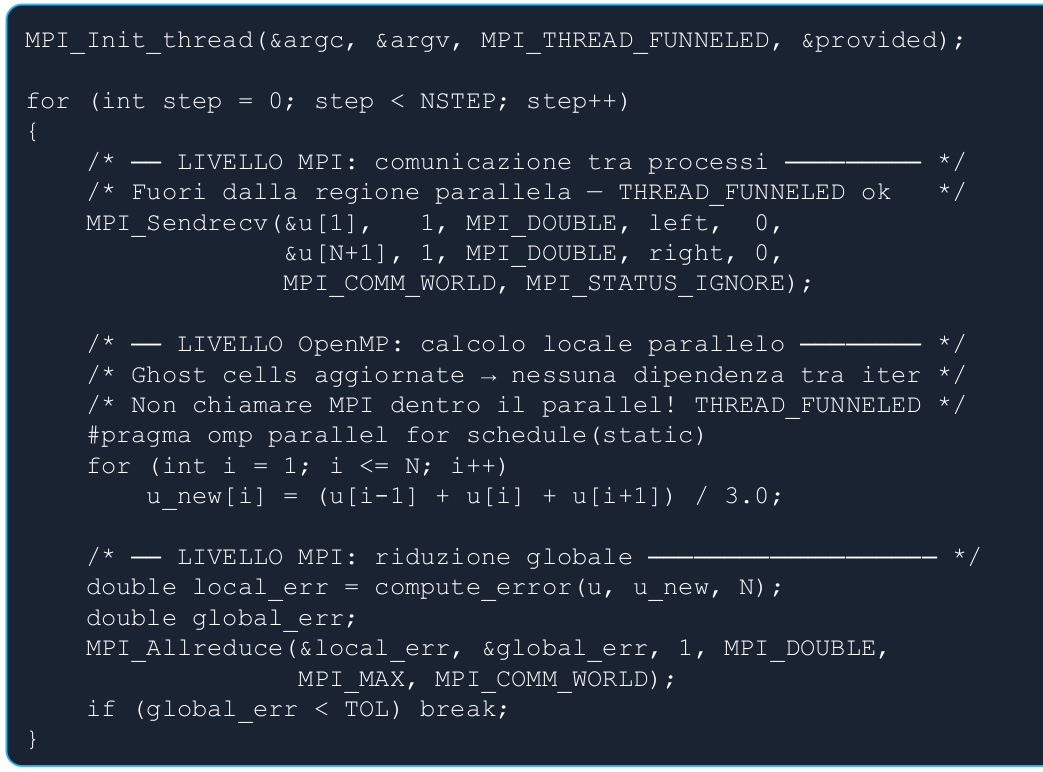
\includegraphics[width=0.8\linewidth]{Images/cap_9/esempio_codice_for.png}
\end{figure}

Il programma segue un ciclo iterativo a tre fasi:
\begin{enumerate}
    \item \textbf{Comunicazione:} Fuori dalla regione parallela, solo il master thread invia/riceve messaggi.
    \item \textbf{Calcolo (Regione OpenMP):} Viene aperto il \texttt{\#pragma omp parallel}. I thread lavorano sui dati locali. È severamente vietato chiamare funzioni MPI in questo blocco.
    \item \textbf{Sincronizzazione globale:} Chiusa la regione parallela, il master thread esegue eventuali riduzioni MPI (es. calcolo dell'errore globale).
\end{enumerate}


\section{Gestione dell'Hardware: Binding e Affinità}

Un programma ibrido raggiunge prestazioni ottimali solo se i thread OpenMP sono esplicitamente legati (pinning/binding) ai core del loro processo MPI. Questo ottimizza l'uso della cache e rispetta l'architettura NUMA (dove gli accessi alla memoria \textit{cross-socket} sono 2-3 volte più lenti).

\subsection{Configurazione e Lancio}
Le variabili d'ambiente istruiscono OpenMP:
\begin{verbatim}
export OMP_NUM_THREADS=4    
# Numero di thread per processo MPI
export OMP_PROC_BIND=close  
# Mantiene i thread e i dati sullo stesso socket NUMA
export OMP_PLACES=cores     
# Assegna un thread per ogni core fisico
\end{verbatim}

Il comando di avvio mappa i processi sull'hardware tramite \texttt{mpirun}:
\begin{verbatim}
mpirun -np 2 
--bind-to socket 
--map-by socket:pe=4 
./programma_ibrido
\end{verbatim}
\textit{Nota: A runtime, si può usare la funzione \texttt{sched\_getcpu()} per stampare l'ID del core e verificare il corretto posizionamento dei thread.}

\subsection{Associazione: Caso di Studio Intel}
In un cluster con nodi \textit{dual-socket} a 6 core ciascuno (12 core per nodo), una mappatura \textbf{Completamente Ibrida} (utilizzando la toolchain Intel) si configura così:
\begin{verbatim}
OMP_NUM_THREADS=12 mpirun -ppn 1 -np 2
 -env KMP_AFFINITY scatter ./a.out
\end{verbatim}
Si generano 12 thread, si alloca 1 processo per nodo (\texttt{-ppn 1}), impegnando in totale 2 nodi (\texttt{-np 2}). \texttt{KMP\_AFFINITY scatter} assicura che i thread siano distribuiti uniformemente sull'hardware.


\section{Build, Linkaggio ed Esecuzione}

Gestire la compilazione richiede l'uso combinato dei tool:
\begin{itemize}
    \item Si compila con il wrapper MPI (es. \texttt{mpicc}) aggiungendo il flag OpenMP (es. \texttt{-fopenmp}). Il linkaggio è generalmente automatico.
    \item I comandi di esecuzione dipendono dal gestore (Slurm, PBS) e sono \textbf{altamente non portabili}. È fondamentale garantire che variabili come \texttt{OMP\_NUM\_THREADS} siano propagate a tutti i processi sui vari nodi.
\end{itemize}

\subsection{Compilare da un singolo sorgente}
Per evitare di mantenere versioni separate (seriale, puramente MPI, ibrido), è prassi usare il preprocessore C/C++. Il simbolo \texttt{\_OPENMP} è definito automaticamente dal compilatore se il flag è attivo, mentre \texttt{USE\_MPI} si può definire manualmente (\texttt{-DUSE\_MPI}).
\begin{verbatim}
int rank = 0;
int size = 1;

#ifdef USE_MPI
    MPI_Init(...);
    MPI_Comm_rank(MPI_COMM_WORLD, &rank);
    MPI_Comm_size(MPI_COMM_WORLD, &size);
#endif
\end{verbatim}
Impostare i default per rank e size garantisce l'esecuzione del codice anche in modalità puramente seriale/OpenMP.


\section{Metodologia: Approccio Multilivello e Pitfalls}

\subsection{Approccio Generale Multilivello}
Per sviluppare un'applicazione ibrida efficiente, si utilizza una tecnica \textit{Top-Down}:
\begin{enumerate}
    \item \textbf{Decomposizione (MPI):} Si distribuisce il dominio globale o i task principali ai vari processi (es. distribuzione della griglia spaziale).
    \item \textbf{Parallelismo locale (OpenMP):} Tramite l'uso di un \textit{profiler}, si individuano gli \textit{hotspot} computazionali. Si applica OpenMP ai cicli interni più intensivi (es. aggiornamento della mesh) bilanciando empiricamente i thread per massimizzare l'efficienza.
\end{enumerate}

\subsection{Cose su cui fare attenzione (Pitfalls)}
\begin{itemize}
    \item \textbf{Overhead di creazione:} L'apertura e chiusura delle regioni OpenMP costa circa $10^4$ operazioni in virgola mobile (flops). Se il lavoro locale è inferiore a questa soglia, OpenMP rallenterà il codice.
    \item \textbf{Comunicazioni concorrenti:} Il livello \texttt{MPI\_THREAD\_MULTIPLE} rende l'architettura del software molto complessa e, purtroppo, molte implementazioni reali delle librerie MPI presentano ancora severi cali di efficienza quando più thread tentano di comunicare contemporaneamente.
\end{itemize}